\chapter{Практическое исследование}





\section{Эксперименты ранжирующими методами}
\label{sec_experiments}

Мы провели три серии экспериментов для разных размеров графа.  Во-первых, мы
рассмотрели небольшие графы из около $20$ вершин, где мы смогли сравнить базовые,
оптимальное в среднем и полуэвристический методы.  Во всех остальных
экспериментах не рассматривался оптимальное в среднем ранжирования, поскольку
оно вычислительно невыполнима для графов большого размера.  Затем мы
проанализировали графы среднего размера из $100$ вершин.  Для таких размеров,
которые ближе к реальным, мы проанализировали базовые и полуэвристический
методы.  В конце мы протестировали методы на графе, взятого из реальных данных
из двух тысяч вершин.





\subsection{Графы маленького размера}

В первом эксперименте мы сгенерировали $32$ разных графа размера $18$.
Активный модуль размера $4$ был выбран равномерно случайным образом.  Значение
$a$ было выбрано равномерно из распределения $U(0, 0,5)$.  Веса вершин
генерировали из соответствующих бета- и равномерных распределений.

Результаты первого эксперимента показаны на рисунке~\ref{fig:smalluni}.  Они
показывают, что метод оптимального в среднем в большинстве случаев работает
одинаково или лучше по сравнению с \emph{BioNet} и немонотонными базовыми
методами (верхние панели).  Полуэвристический метод работает аналогично хорошо
по сравнению с оптимальным (нижняя левая панель) и лучше, чем метод
\emph{BioNet}.

\begin{figure}
    \centering
    \begin{tabular}{@{}cccc@{}}
        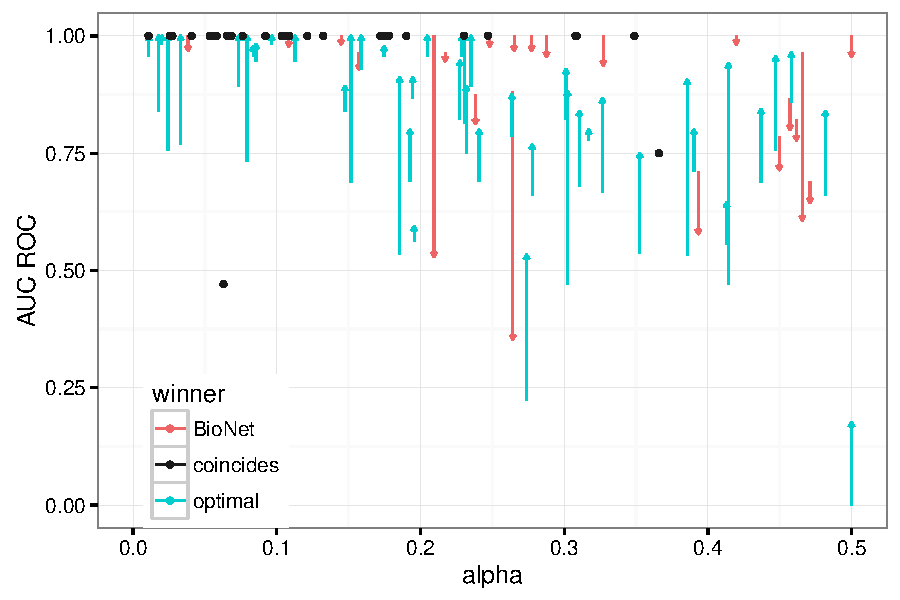
\includegraphics[width=3.2in]{su_ob.pdf} &
        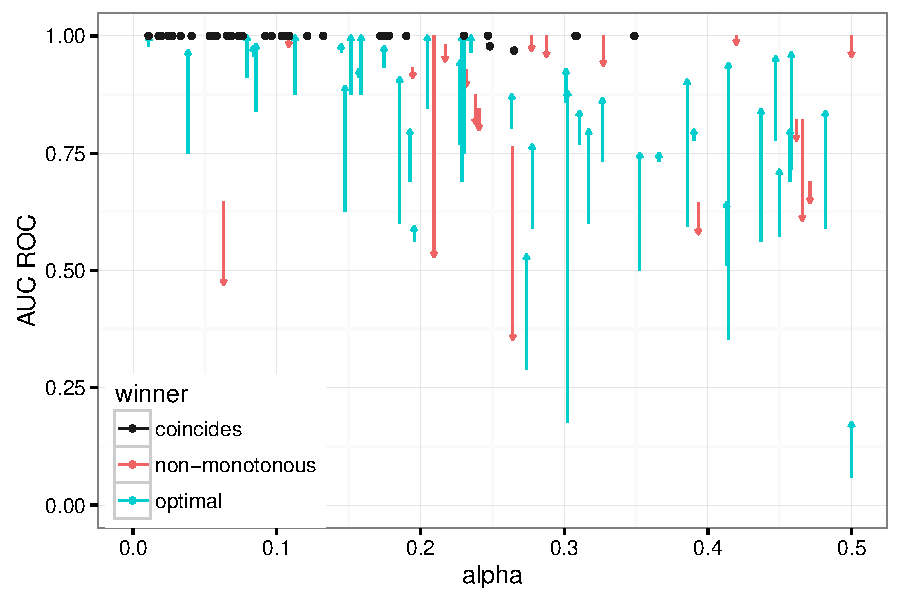
\includegraphics[width=3.2in]{su_on.pdf} \\
        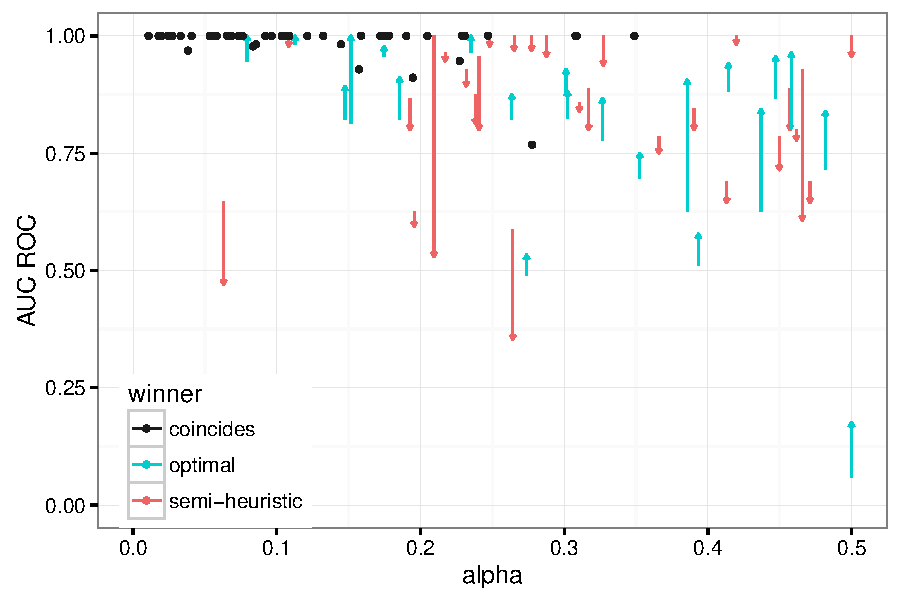
\includegraphics[width=3.2in]{su_os.pdf} &
        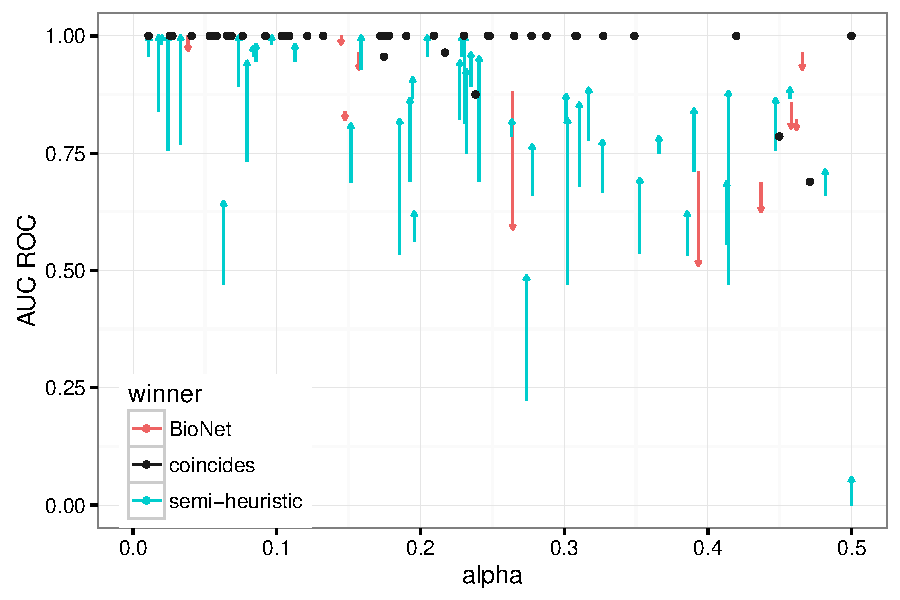
\includegraphics[width=3.2in]{su_sb.pdf}    
    \end{tabular}
    \caption{
        Модульные значения \emph{AUC} для графа размера $18$.  Присутствуют
        следующие методы: оптимальный в среднем, полуэвристический,
        \emph{BioNet} и немонотонный.  На каждой панели показано сравнение двух
        методов.  Одна стрелка соответствует одному эксперименту, концы стрелки
        соответствуют значениям \emph{AUC} первого и второго метода. Цвет
        зависит от того, какой метод работает лучше.  Настоящие активные модули
        были отобраны из равномерного распределения.
    }%
    \label{fig:smalluni}%
\end{figure}

Распределение активных модулей может быть неравномерным в реальных данных,
поэтому мы также провели эксперимент с таким неравномерным распределением
(подробнее в~\ref{sec_details}).  Помимо четырех рассмотренных методов, мы
использовали метод оптимального в среднем, параметризованный реальным
эмпирическим распределением модулей.

Результаты этого эксперимента показаны на рисунке~\ref{fig:smallnon}.  Ситуация
аналогична предыдущему эксперименту с полуэвристическим методом, он почти как
метод оптимальный в среднем и лучше базовых методов.  Однако полуэвристический
метод работает хуже, чем метод оптимального в среднем, параметризированный
распределением реальных модулей.

\begin{figure}
    \centering
    \begin{tabular}{@{}cccc@{}}
        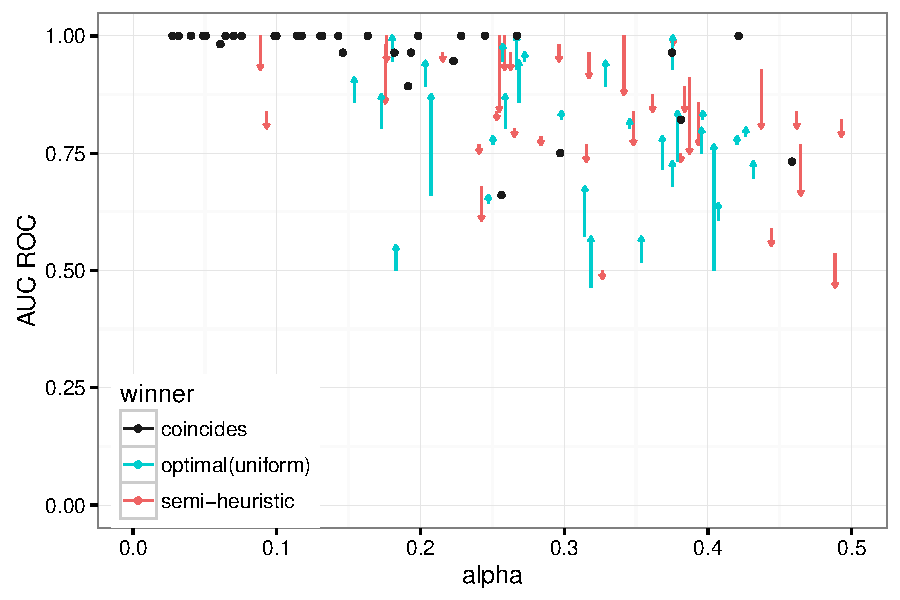
\includegraphics[width=3.2in]{sn_uos.pdf} &
        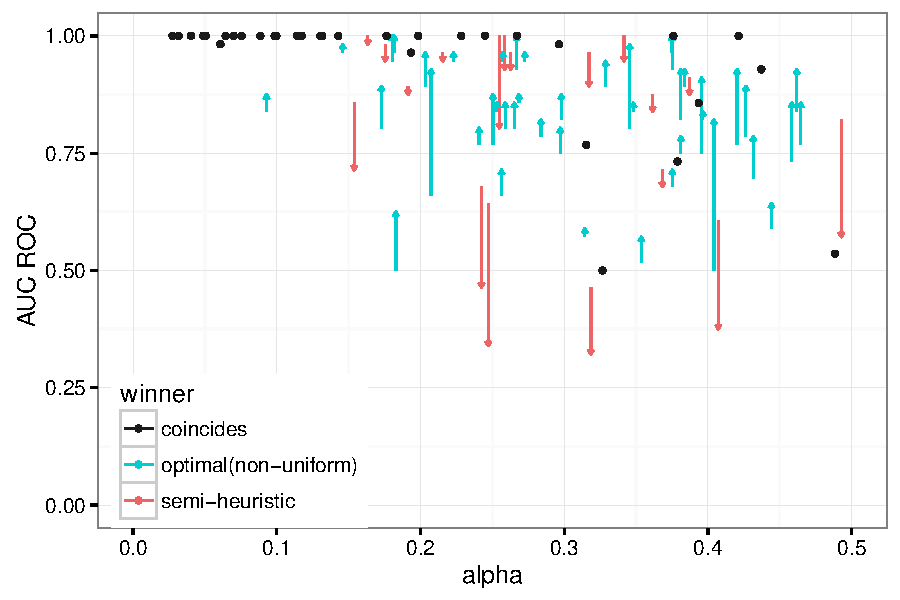
\includegraphics[width=3.2in]{sn_nos.pdf} \\ 
        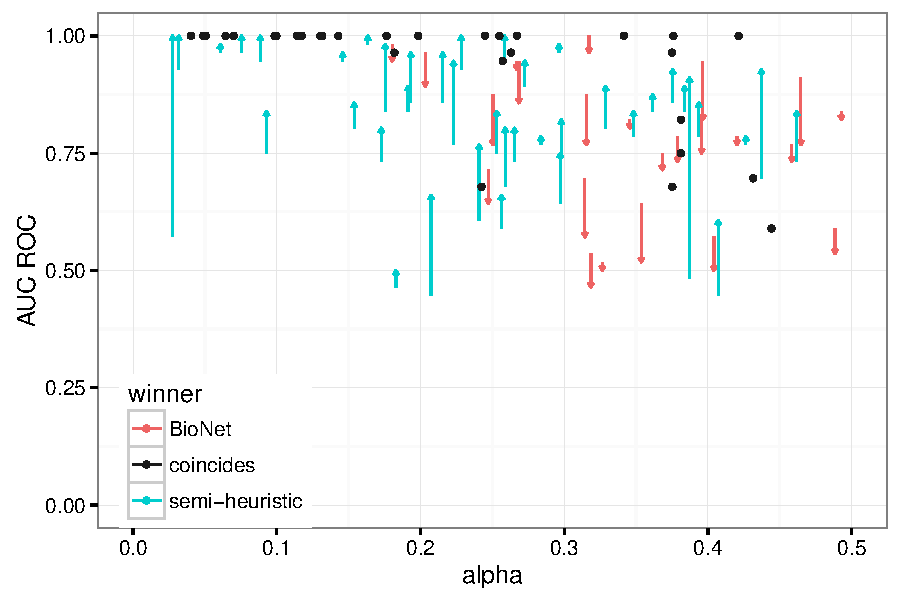
\includegraphics[width=3.2in]{sn_sb.pdf} &
        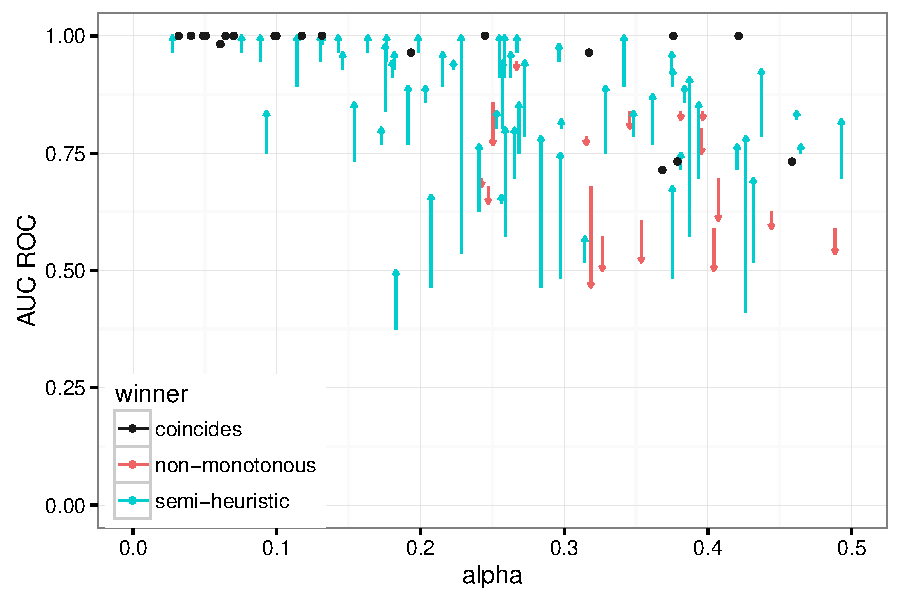
\includegraphics[width=3.2in]{sn_sn.pdf}    
    \end{tabular}
    \caption{
        Модульные значения \emph{AUC} для графа размера $18$ для настоящих
        активных модулей, отобранных из неравномерного распределения.
        Приводятся следующие методы: оптимальный в среднем, оптимальный
        в среднем параметризированное действительным распределением,
        полуэвристический, BioNet и немонотонный.
    }%
    \label{fig:smallnon}%
\end{figure}





\subsection{Графы среднего размера}

Как и в предыдущем разделе, мы создали $32$ разных графа размера $100$.
Размер активного модуля был отобран равномерно от $5$ до $25$.

На этих размерах графа использование метода оптимального в среднем становится
неосуществимым, поэтому мы исключили его из анализа.  Среднее время выполнения
полуэвристического метода составляло $146$ секунд.

Результаты эксперимента приведены на рисунке~\ref{fig:med}.  Почти во всех
случаях полуэвристическое ранжирование работало лучше, чем базовые методы
\emph{BioNet} и немонотонный метод.

\begin{figure}
    \centering
    \begin{tabular}{@{}cccc@{}}
        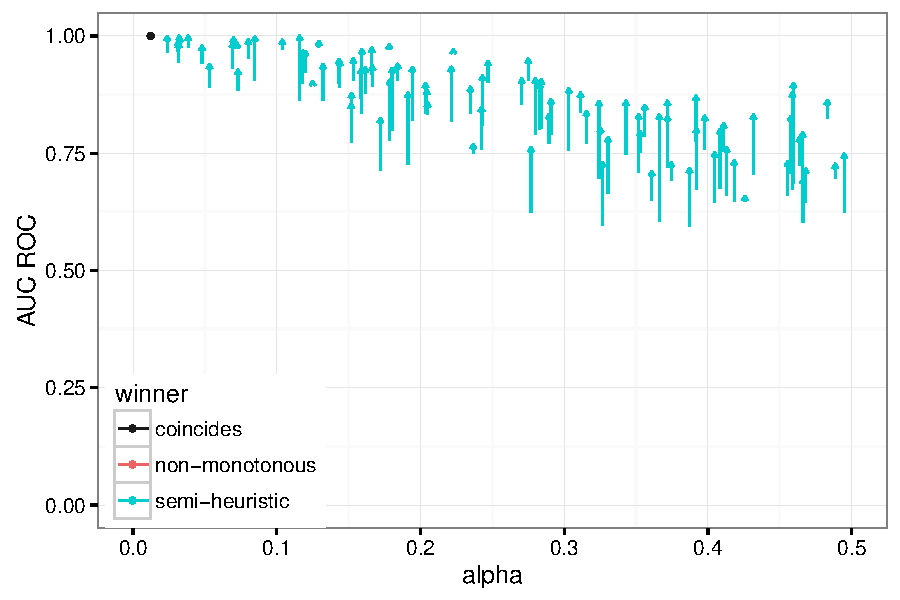
\includegraphics[width=3.2in]{mn_sn.pdf} &
        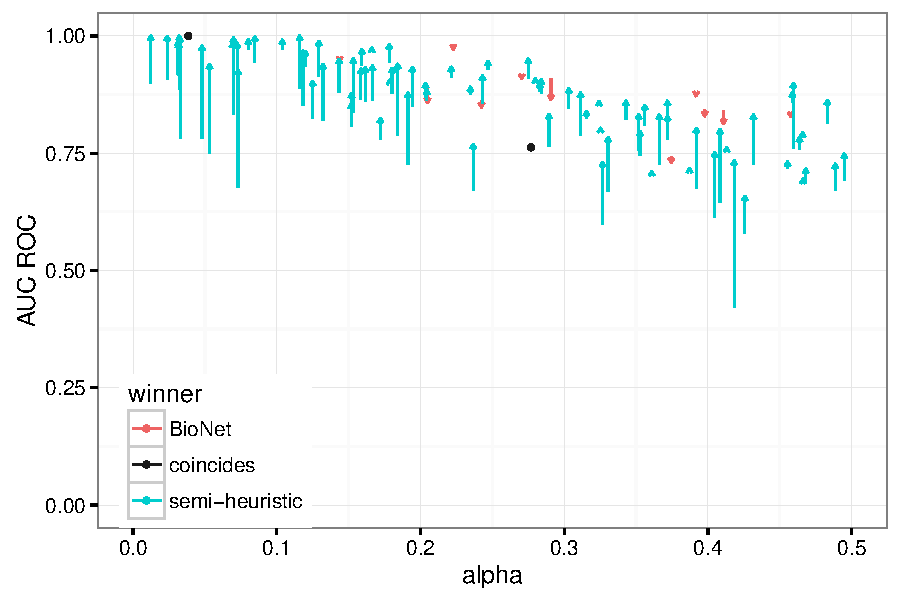
\includegraphics[width=3.2in]{mn_sb.pdf}  
    \end{tabular}
    \caption{
        Модульные значения \emph{AUC} для графа размера $100$. Представлены три
        метода: полуэвристический, \emph{BioNet} и немонотонный.
    }%
    \label{fig:med}%
\end{figure}





\subsection{Графы большого размера}

В последнем эксперименте мы проанализировали эффективность предложенного
полуэвристического метода на большом графе. Для этого эксперимента мы
использовали граф белок-белковых взаимодействий на примере пакета
BioNet~\cite{Beisser2010}.  Этот граф имеет $2089$ вершин и $7788$ ребер.
Активным модулем в этой сети был подграф размером $50-250$.

Результаты эксперимента показаны на рисунке~\ref{fig:lar}. Как и для графов
средних размеров, полуэвристический метод  работает лучше, чем оба базовых
метода. С другой стороны, время работы метода значительно увеличилось примерно
до шести часов.

\begin{figure}
    \centering
    \begin{tabular}{@{}cccc@{}}
        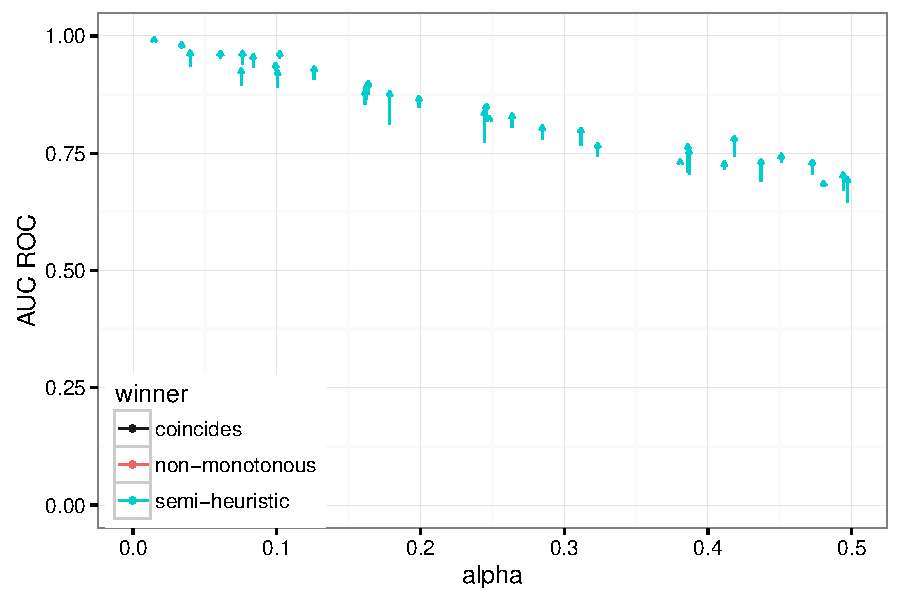
\includegraphics[width=3.2in]{ln_sn.pdf} &
        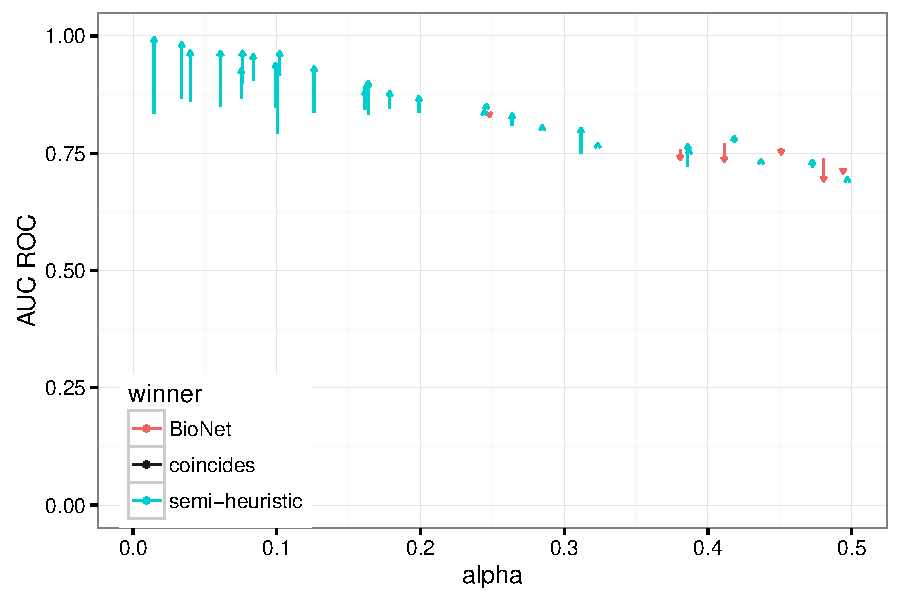
\includegraphics[width=3.2in]{ln_sb.pdf}    
    \end{tabular}
    \caption{
        Модульные значения \emph{AUC} для реального графа взаимодействий
        протеин-протеин.  Представлены три методы: полуэвристический,
        \emph{BioNet} и немонотонный.
    }%
    \label{fig:lar}%
\end{figure}





\subsection{Генерация графов для экспериментов}
\label{sec_details}

Для имитации реальных сетевых графов для экспериментов были сгенерированы
безмасштабные сети (\emph{scale-free network}).  Для генерации мы использовали
существующую реализацию алгоритма Барабаси-Альберта из \emph{R}-пакета
\emph{igraph}.

Для выборки подграфа данного размера мы использовали следующую процедуру.
Пусть $G = (V, E)$ -- связный граф, $k$ -- требуемый размер активного модуля
и $M$ -- множество вершин генерируемого случайного активного модуля. В начале
$M$ пусто, добавим в $M$ случайную вершину из графа $G$.  Затем мы выберем
одну из смежных вершин $M$, которая еще не принадлежит $M$, и добавляем ее.
Этот шаг повторяется до тех пор, пока $M$ не будет иметь размер $k$.





\section{Эксперименты методом оценки вероятности вхождения вершины}

Сначала рассмотрим <<игрушечный>> пример. Мы создали случайный граф $G$ на $30$
вершинах и $65$ ребрах.  Затем мы выбрали активный модуль $M$ из $9$ вершин
случайным образом и породили веса из бета-распределения $\beta(0,2, 1)$ для
вершин из $M$ и из равномерного распределения для всех других вершин.  Для
такого <<игрушечного>> примера мы можем как вычислить вероятности $P(v \in
M \mid W=w)$ непосредственно из \eqref{eq:graphprobs}, так и оценить их как
$P(v \in M \mid W=w)$, используя наш подход \emph{MCMC}.  Мы выполняем $10^6$
итераций алгоритма Метрополиса-Гастингса.  Оценки очень точно аппроксимировали
реальные вероятности с среднеквадратичной ошибкой равной $2 \cdot 10^{-3}$.
Отметим также, что ранжирование вершин на основе оценок $P(v \in M \mid W=w)$
то же самое, что ранжирование на основе истинных вероятностей.
Производительность ранжирования обычно измеряется с помощью кривой \emph{ROC}
и ее \emph{AUC}. Для обоих фактических и оценочных вероятностей \emph{AUC} был равен
$0,92$.

\begin{figure}
    \centering
    \begin{tabular}{@{}cccc@{}}
        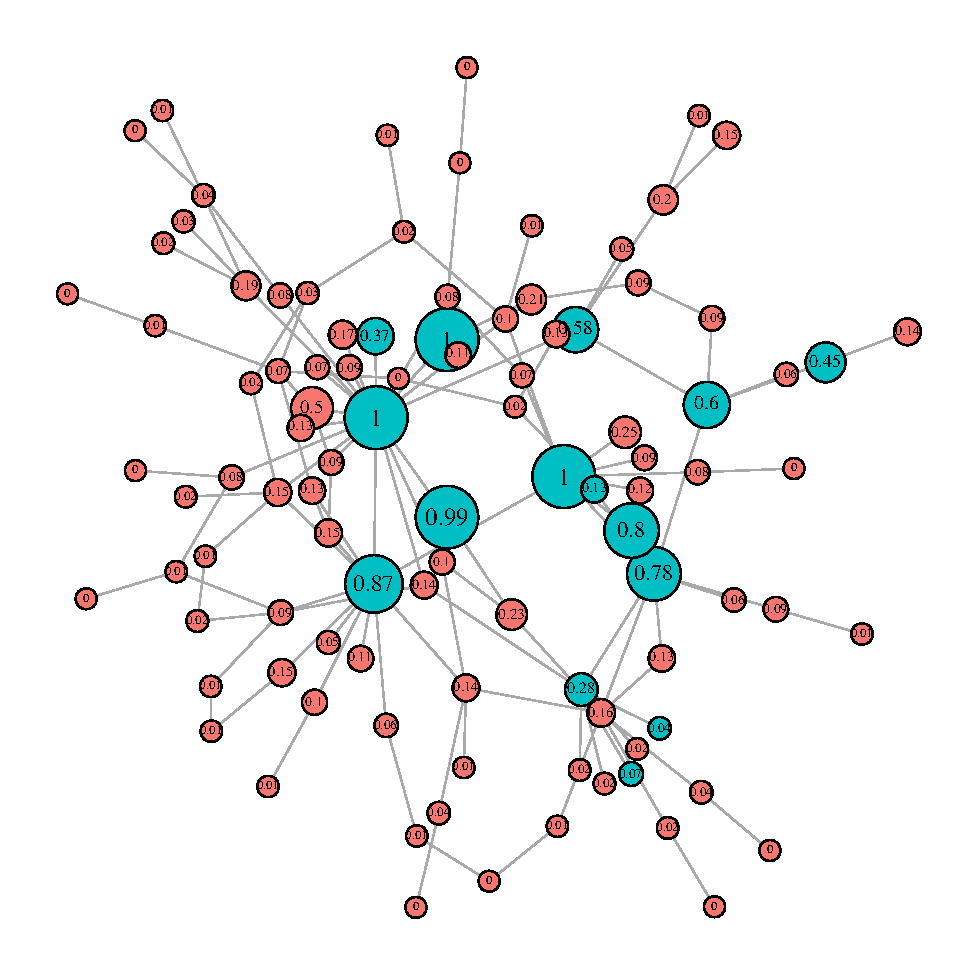
\includegraphics[width=6.5in]{graph_prob.pdf}
    \end{tabular}
    \caption{
        Вероятности вхождения вершин в активный модуль для симулированного
        графа размера $100$.  Активный модуль был выбран случайным образом из
        множества подграфов размера $15$ и параметр бета-распределения $a
        = 0,2$.  Вероятность вершины измеряется на основе $1000$ независимых
        образцов \emph{MCMC} с $500$ итерациями.  Вершины из активного модуля
        окрашены синим цветом, а все остальные вершины красным цветом.  Надпись
        на вершинах означает вероятность вхождения с точностью до второго знака
        после запятой.  Чем больше размер вершины, тем высока ее вероятность.
    }%
    \label{fig:graph_prob}%
\end{figure}


Дальше мы сравнили наш \emph{вероятностный} подход с другими методами на симулированных
данных.  Здесь мы рассмотрели $100$ случайных экземпляров (например,
рисунок~\ref{fig:graph_prob}). Для каждого экземпляра был сгенерирован
случайный \emph{безмасштабный} (\emph{scale-free}) граф из $100$ вершин.  Затем
мы сгенерировали активные модули в два этапа:
1) размер модуля был равномерно выбран от $5$ до $25$ и
2) модуль был выбран равномерно случайным образом из всех связных подграфов
   выбранного размера.  Веса вершин генерировались из смеси бета-равномерного
   распределения со значениями параметра $a$, выбранного из интервала $[0,01,
   0,5]$. Показатели \emph{AUC} для ранжирования, полученные четырьмя
   проверенными методами, показаны на рисунке~\ref{fig:comp}.  Для всех
   значений $a$, предложенный нами метод показал результат значительно выше по
   сравнению со всеми тремя базовыми методами.

\begin{figure}
    \centering
    \begin{tabular}{@{}cccc@{}}
        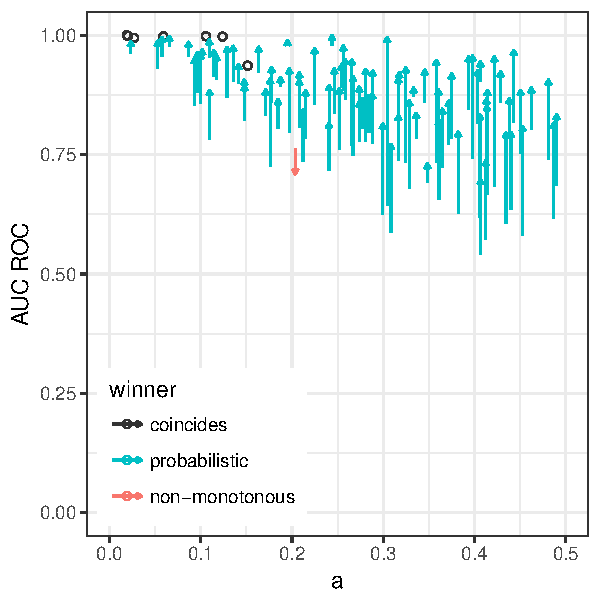
\includegraphics[width=2.1in]{probabilistic_vs_non-monotonous.pdf} &
        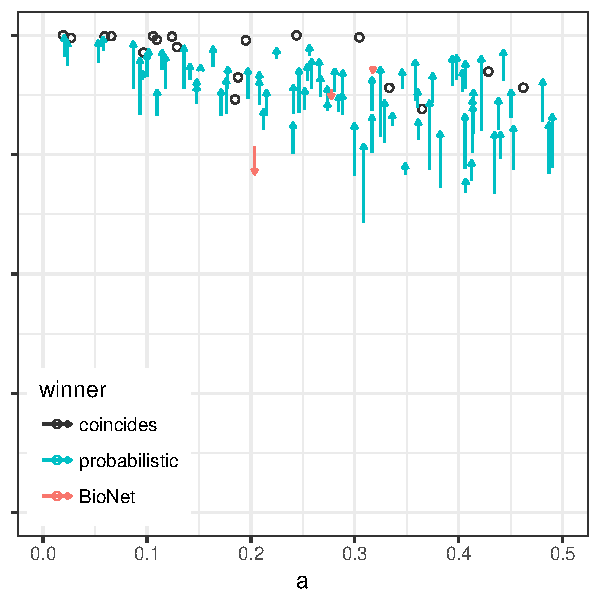
\includegraphics[width=2.1in]{probabilistic_vs_bionet.pdf} & 
        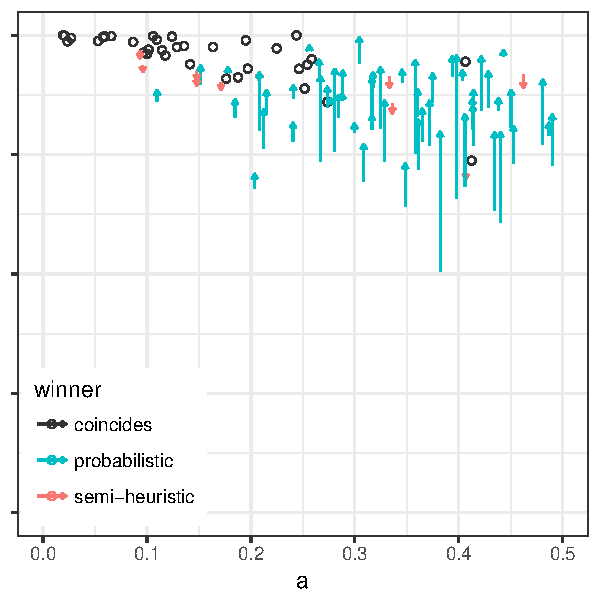
\includegraphics[width=2.1in]{probabilistic_vs_shmyak.pdf}
    \end{tabular}
    \caption{
        \emph{AUC ROC} значения ранжирований симулированных графов размера $100$.
        Предложенный нами метод ражирования вероятностный сравнивается со следующими
        методами: ранжирование по входным весам, ранжирование на основе
        \emph{BioNet} и полуэвристическое ранжирование
        из~\cite{Isomurodov2017}.  Одна стрелка соответствует одному
        эксперименту.  Концы стрелки указывают на оценку \emph{AUC ROC}
        вероятностного ранжирования.  Цвет зависит от того, какой метод показал
        лучший \emph{AUC ROC}.
    }%
    \label{fig:comp}%
\end{figure}

Затем мы рассмотрели производительность \emph{MCMC} на реальном графе
белок-белковых взаимодействий.  Мы использовали граф с $2034$ вершинами
и $8399$ ребрами, построенный в~\cite{Dittrich2008a} для диффузного большого
набора данных \emph{В}-клеточной лимфомы.  Мы выбрали активный модуль
равномерно случайным образом из множества связных подграфов с $200$ вершинами.
Веса вершин в активном модуле генерировались из бета-распределения $\beta(0,25,
1)$.  Во-первых, мы рассмотрели поведение значений логарифмического
правдоподобия для образцов во время одного запуска \emph{MCMC}
(рисунок~\ref{fig:auclog}, зеленая линия).  Этот график показывает, что
значение логарифмического правдоподобия стабилизируется после примерно $25000$
итераций.  Таким образом, мы можем оценить время смешивания $T$ метода
\emph{MCMC} как $25000$ для этого случая.  Затем мы проверили, что для оценки
вероятностей вершин достаточно $25000$ итераций.  Для разных значений $T'$ мы
рассчитали значения \emph{AUC ROC} для ранжирования на основе $1000$ независимых
запусков \emph{MCMC} для $T$ итераций (рисунок~\ref{fig:auclog}, красная
линия).  Результаты показывают, что действительно $25000$ итераций достаточно
для достижения высоких значений \emph{AUC ROC}, а фаза насыщения начинается еще
раньше.  В конце, мы сравнили ранжирование на один длинный запуск \emph{MCMC}
и на $1000$ независимых выборок (рисунок~\ref{fig:auclog}, синяя линия).
В течение одного долгого запуска мы оценивали вероятности, используя все
сгенерированные образцы \emph{MCMC}, за исключением первых $25000$.  Можно
видеть, что значения \emph{AUC ROC} насыщаются после примерно $50000$ итераций
\emph{MCMC}, что оправдывает использование одного долгого запуска \emph{MCMC}.
Практически это означает, что хорошие оценки вероятности могут быть достигнуты
очень быстро, учитывая, что $100000$ итераций \emph{MCMC} заняли около одной
минуты на ноутбуке.

\begin{figure}
    \centering
    \begin{tabular}{@{}cccc@{}}
        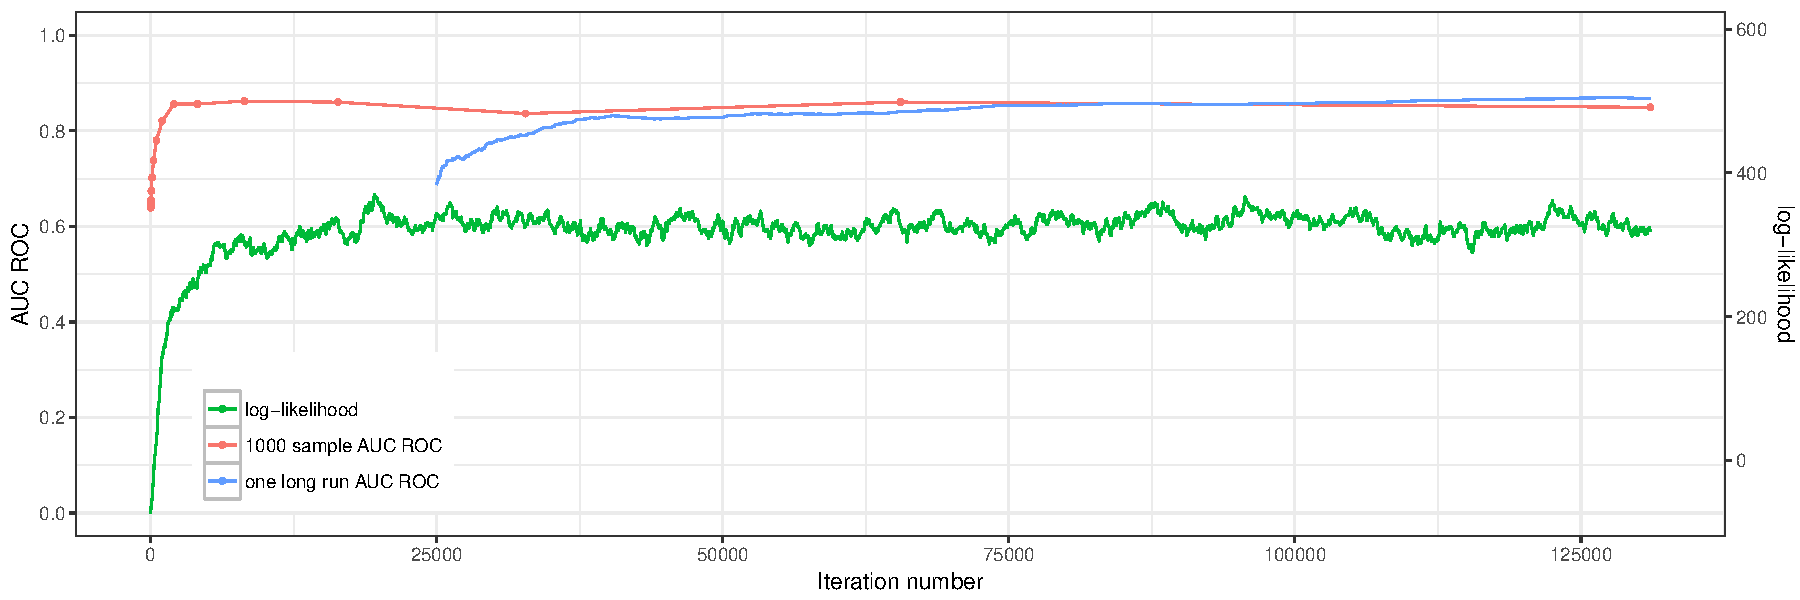
\includegraphics[width=6.5in]{auc_loglikelihood.pdf}
    \end{tabular}
    \caption{
        Поведение значения логарифмического правдоподобия подграфа
        и ранжирования \emph{AUC ROC} в зависимости от количества итераций
        \emph{MCMC}.  В качестве $G$ используется реальный граф белок-белковых
        взаимодействий из $2034$ вершин, модуль из $200$ вершин выбирается
        равномерно случайным образом.  Зеленая линия: значения логарифмического
        правдоподобия для подграфов $S_i$, сгенерированных во время одного
        запуска \emph{MCMC}.  Красная линия: значения \emph{AUC ROC} для
        ранжирования на основе $1000$ независимых образцов \emph{MCMC}
        в зависимости от выбранной оценки времени смешивания.  Синяя линия:
        значения \emph{AUC ROC} для ранжирования на основе одного запуска
        \emph{MCMC}, рассчитанного для всех выборок $S_i$ для $i > 25000$.
    }%
    \label{fig:auclog}%
\end{figure}

Еще одним из экспериментов была проверка на \emph{FDR}.  Мы рассмотрели $20$
разных экземпляров, где в качестве графа выбрали граф белок-белковых
взаимодействий из предыдущего эксперимента.  Для каждого экземпляра выбрали
значение параметра $a$ бета-распределения равномерно случайным образом из
отрезка $[0, 0,5]$ и также выбрали случайно активный модуль из множество
связных графов с $200$ вершинами.  Для каждого экземпляра запустили $1000$
независимых \emph{MCMC} с $25000$ итераций, вычислили вероятности вхождения
вершин в активный модуль и на основе вероятностей построили вероятностное
ранжирование.  Далее на каждый запрос с заданным \emph{FDR}, мы находили
множество вершин полученных из префикса ранжирования.  Выбирали префикс
максимальной длины, чтобы средняя ошибка у всех вершин этого префикса не
превышала заданный \emph{FDR}.  Для всех экспериментов увидели, что настоящий
\emph{FDR} не сильно отличается от запрашиваемого \emph{FDR} (например, для $a
= 0,25$ рисунок~\ref{fig:fdr}).

\begin{figure}
    \centering
    \begin{tabular}{@{}cccc@{}}
        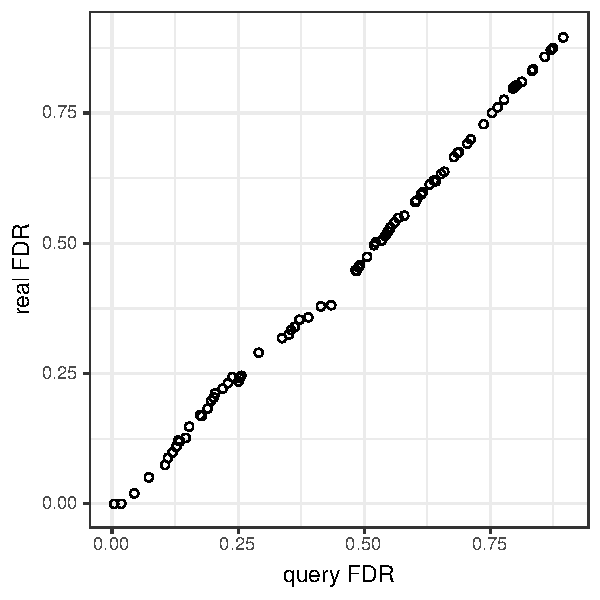
\includegraphics[width=4.0in]{plot-fdr.pdf}
    \end{tabular}
    \caption{
        Каждая точка -- это подграф со средней ошибкой (вычисляется через
        вероятности вершин, посчитанных с помощью метода \emph{MCMC}) не
        больше, чем значение $x$-координаты и с настоящим \emph{FDR}, равным
        значению $y$-координаты.  По оси $x$ -- \emph{FDR} запрос, по оси $y$
        -- настоящий \emph{FDR}.  Этот эксперимент для графа, полученный из
        белок-белковых взаимодействий.  Модуль выбран из множеств связных
        подграфов размера $200$ случайным образом. Параметр бета-распределения
        $a=0,25$.
    }%
    \label{fig:fdr}%
\end{figure}

Хотя мы оценили параметры смеси бета-равномерного распределения
с инструментом~\cite{Beisser2010}, мы протестировали наш метод на надежность от
ошибок оценки параметров смеси.  Как и раньше, мы выбрали граф белок-белкового
взаимодействий и активный модуль равномерно случайным образом из множества
связных подграфов размером $200$ вершин.  Веса вершин в активном модуле
генерировались из бета-распределения $\beta(0,25, 1)$.  Затем мы запустили
алгоритм \emph{MCMC}, предполагая количество вершин в модуле $k = 50, 100, 150,
200, 300, 400$ и параметр бета-распределения $a = 0,15, 0,2, 0,25, 0,3,
0,35, 0,4$.  Методы хорошо выполняются для этих неточных значений параметров
  (таблицу~\ref{tab:bla}).

\begin{table}[!htb]
    \captionsetup{justification=centering}
    \caption{
        Поведение алгоритма \emph{MCMC} в зависимости от неточно заданных
        параметров \emph{BUM} распределения: (\subref{tab:lambda}) количество
        вершин в модуле и (\subref{tab:a}) параметр формы $a$. Результаты
        усредняются на $10$ запусков.
    }
    \label{tab:bla}
    \begin{subtable}{.5\linewidth}
        \caption{}
        \begin{tabular}{c|c}
                Размер модуля &   \emph{AUC ROC} \\
                \hline
                50 & 0.7855947 \\
                100 & 0.8480398 \\
                150 & 0.8686694 \\
                200 & 0.8674064 \\
                300 & 0.8697938 \\
                400 & 0.8669445 \\
        \end{tabular}
        \label{tab:lambda}
    \end{subtable}%
    \begin{subtable}{.5\linewidth}
        \caption{}
        \begin{tabular}{c|c}
            Параметр $a$ &   \emph{AUC ROC} \\
            \hline
            0.15 & 0.8685988 \\
            0.2  & 0.8686608 \\
            0.25 & 0.8676020  \\
            0.3 & 0.8694082 \\
            0.35 & 0.8618193 \\
            0.4 & 0.8639373 \\
        \end{tabular}
        \label{tab:a}
    \end{subtable}
\end{table}





\section{Обсуждение}

Настоящее исследование мы рассматриваем как проблему мягкой классификации
и предлагаем метод оценки вероятностей принадлежности каждой вершины
к активному модулю.  Наш метод показывает высокую точность моделирования данных
(рисунки~\ref{fig:comp} и~\ref{fig:auclog}) и выполняется быстро даже на графах
большого размера (например, нам удалось обработать реальный граф белок-белковых
взаимодействий из~\cite{Dittrich2008a}, который содержит $2034$ вершин,
примерно за минуту).

Мы показываем, что  метод \emph{MCMC} способен достичь <<стабилизированной>>
фазы в разумном числе итераций, что является одной из основных проблем при
разработке методов Монте-Карло по схеме марковской цепи.  Мы также показываем,
что одного длинного запуска \emph{MCMC} достаточно для точного ранжирования
вершин, что делает метод очень практичным с точки зрения производительности.
На примерах, которые мы рассмотрели, потребовалось меньше нескольких минут для
достижения высокой точности, и есть еще место для оптимизации, чтобы сделать
этот метод еще быстрее.

В то время как здесь мы обсудили как вычислить вероятности принадлежности
к активному модулю только для отдельных вершин (для оценки важности отдельных
генов), наш метод можно также использовать для оценки таких вероятностей для
ребер (для оценки важности конкретных взаимодействий) или даже для оценки
небольших подграфов.  Кроме того, полученные вероятности позволяют ранжировать
вершины и непосредственно вычислять \emph{FDR} для любого модуля-кандидата.

Отметим, что хотя мы предполагаем в нашей модели, что веса вершин графа
распределены в соответствии с распределением \emph{BUM}, алгоритм может быть
легко адаптирован для любого разумного распределения веса.  Кроме того, в то
время как в текущей версии мы используем оценку максимального правдоподобия
из~\cite{Beisser2010} для оценки параметров распределения \emph{BUM}, в дальнейшей
разработке мы можем модернизировать алгоритм~\ref{alg:mh}, чтобы более точно
оценить эти параметры.  Мы также отмечаем, что наш метод является надежным, то
есть показывает высокую точность, даже если параметры отличаются от фактических
значений (таблица~\ref{tab:bla}).





\section{Детали реализации}
\emph{МСМС} метод был реализован на языке программирования \emph{C++}.
Реализованная структура графа хранит исходный граф и массивы внутренних
и соседних вершин связного подграфа.  На этапе инициализации генерируется
связный подграф заданного размера и обновляются массивы внутренних и соседних
вершин.  Далее, совершается запрашиваемое количество итераций, каждая итерация
это шаг действий.  Каждый шаг представляет из себя удаление и добавление
случайной вершины в связный подграф из массивов внутренних и соседних вершин
соответственно.  Далее, проверяется связность подграфа с помощью обхода
в ширину, если подграф окажется несвязным, то шаг считается неудачным.  Также
в каждом шаге пересчитывается лайклихуд и массив соседних вершин и считается
величина $\rho$. С вероятностью $1 - \rho$ каждый шаг считается неудачным (
рисунок~\ref{recombiter}).  Если шаг считается неудачным, то все изменения,
сделанные во время этого шага отклоняются.  Здесь вычислительная часть является
проверкой на связность графа и обновление массива соседних вершин.  Проверка на
связность графа работает за $O(|S|)$, где $S$ - это связный подграф.
Обновление массива соседних вершин выполняется за время
$O(|nei(v_+)|+|nei(v_-)|)$.



\section{На реальных данных}

Мы применили наш метод к набору данных \emph{диффузной B-крупноклеточной
лимфомы} (\emph{Diffuse large B-cell lymphoma}, \emph{DLBCL}) и к графу
белок-белковых взаимодействий построенному в~\cite{Dittrich2008a}.  Данные
экспрессии были взяты из исследования \emph{DLBCL} от~\cite{Alizadeh2000}.
\emph{P}-значения в наборе данных \emph{DLBCL} являются результатом
дифференциальной экспрессии между двумя опухолевыми подтипами, лимфома из
\emph{В}-клеток герминальногоцентра \emph{(GCB) DLBCL} и активированного
\emph{B}-клетки крови \emph{(ABC) DLBCL}. Обратите внимание, что с реальными
данными размер активного модуля, оцененный по методу, предложенному
в~\cite{Dittrich2008a}, имеет тенденцию быть слишком большим (до $50\%$ от
всего графа). Наш метод позволяет справляться с этой проблемой, корректируя
оценки правдоподобия как в~\cite{Dittrich2008a}. Модули выделенный с помощью
предложенного метода ранжирования по вероятности показано на рисунке~\ref{fig:bird-fill}.
\begin{figure}
    \centering
    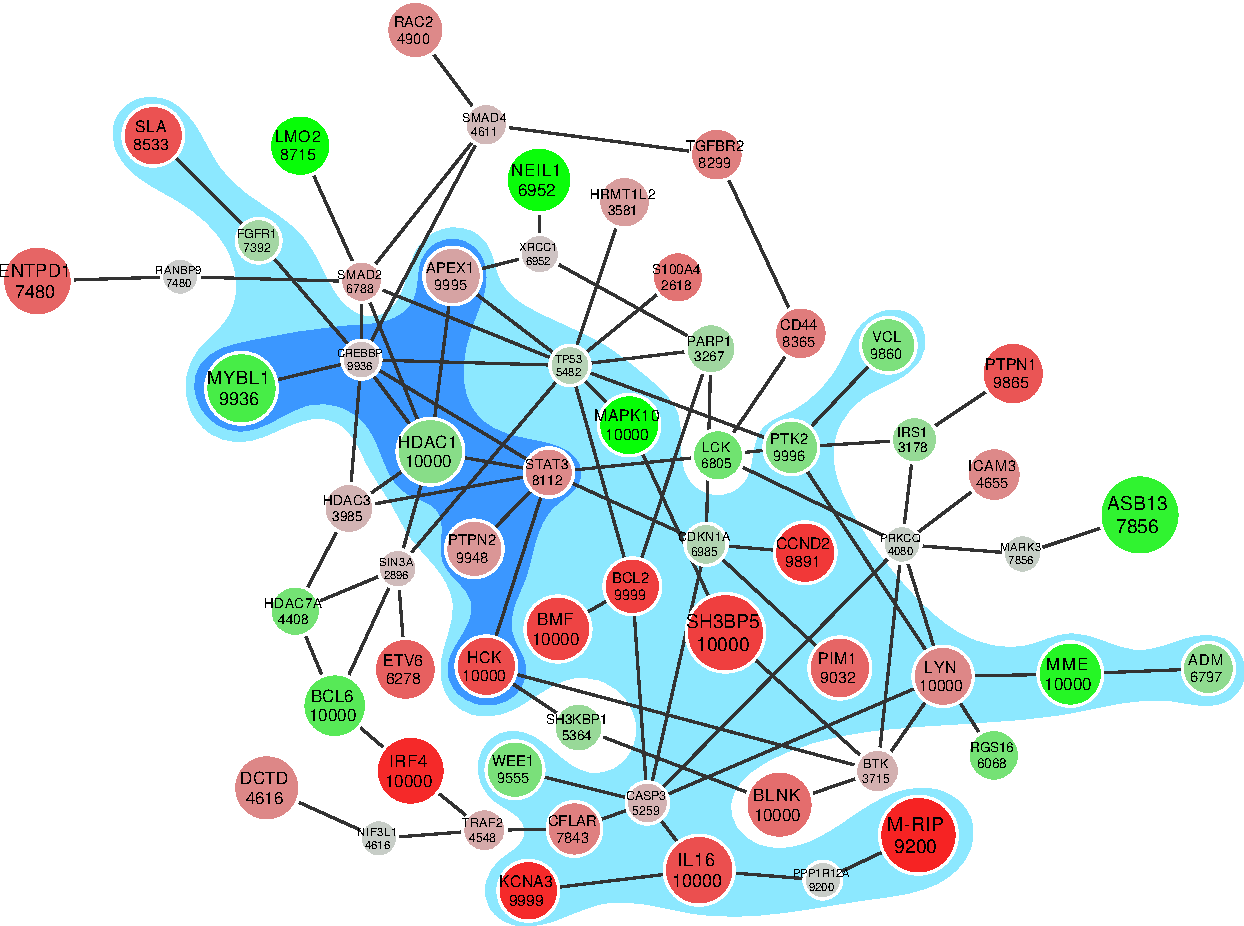
\includegraphics[width=\textwidth]{bird-fill.pdf}
    \caption{
        Подграф индуцированный из вершин с вероятностью не ниже $0,25$ из
        запуска метода \emph{MCMC}.  Сильные оттенки красного или зеленого
        цвета соответствуют более значимым вершинам по \emph{P}-значениям.
        Небольшой подграф темно синего и большой подграф голубого цвета имеют
        \emph{FDR} $0,05$ и $0,1$ соответственно.
    }%
    \label{fig:bird-fill}%
\end{figure}





\chapterconclusion
Была поставлена серия экспериментов для сравнения следующих методов ранжирования:
немонотонной, BioNet, оптимального в среднем и полуэвристического.  Результаты
экспериментов показали, что полуэвристическое ранжирование работает так же, как
и оптимальное в среднем и лучше чем остальные два метода.

Был поставлен эксперимент на сходимость MCMC метода оценки вероятности вершин.
Эксперимент для сравнения метода ранжирования на основе вероятностей с другими
методами ранжирования показал, что первый работает всегда лучше, чем остальные
невероятностные ранжирования.
